Konvoluční neuronové sítě existují již řadu let, ale standardem pro úlohy rozpoznání vzoru v~oboru zpracování obrazu se staly až v~posledních letech. Je to zapříčiněno zejména vyšším výpočetním výkonem počítačů a~velkému množství obrázků a~jimi tvořených datových sad, na kterých je možné tyto neuronové sítě trénovat.

%%%%%%%%%%%%%%%%%%%%%%%%%%%%%%%%%%%%%%%%%%%%%%%%%%%%%%%%%%%%%%%%%%%%%%%%%%%%%%%%%%%%%%%%%%%

\section{Konvoluční neuronové sítě}
\label{cnnTeorie}
Při studiu jsem vycházel z~\cite{CNN, CVmodernApproach}. Hlavní rozdíl mezi konvolučními a~klasickým umělými neuronovými sítěmi je v~tom, že konvoluční sítě jsou používány zejména pro účely rozpoznání vzorů v~oboru zpracování obrazu. Největší nevýhodou umělých neuronových sítí pro výpočet obrazových dat je jejich problém s~vysokou výpočetní složitostí -- dokáží si poradit pouze s~obrázky s~jedním kanálem a~malým rozlišením. Pro komplexnější obrazové vstupy by taková neuronová síť byla příliš velká pro efektivní učení.

\subsection*{Architektura}
Konvoluční neuronové sítě se skládají ze třech typů vrstev. Konvolučních, pooling (sdružovacích) a~plně propojených. První vrstva se nazývá vstupní a~poslední výstupní, mezi nimi se nacházejí vrstvy skryté. Podle \cite{CNN} je postup zpracování jednoho snímku následovný:

\begin{enumerate}
	\item Hodnoty jednotlivých pixelů snímku se uloží do vstupní vrstvy
	\item \textbf{Konvoluční vrstva} určí hodnoty jednotlivých neuronů. Ty jsou dány konvolucí jádra (vah) a~lokální části vrstvy (zvané jako receptivní pole neuronu), se kterou je neuron spojen. Přenosová funkce umístěná za konvoluční vrstvou (např. ReLU\footnotemark) slouží k~provedení aktivací pro každý prvek z~předchozí vrstvy.
	\footnotetext{ReLU -- \emph{Rectified Linear Unit} (rektifikovaná lineární jednotka).}
	\item \textbf{Sdružovací vrstva} poté provede tzv. \emph{downsampling}, tedy podvzorkování (snížení počtu vzorků -- informace), a~to buď za pomoci maximalizace či průměrování okolí pixelu a~výsledkem je pouze jedna hodnota. To slouží ke zmenšení velikosti dané vrstvy.
	\item \textbf{Konvoluční} a \textbf{sdružovací} vrstvy se mohou opakovat. Hluboké konvoluční neuronové sítě se zpravidla skládají z několika skrytých konvolučních vrstev.
	\item Nakonec \textbf{plně-propojená vrstva} vyprodukuje skóre (pravděpodobnosti) jednotlivých tříd z aktivací, sloužící ke klasifikaci.
\end{enumerate}

Proces zpracování konvoluční neuronovou sítí popsaný výše lze vidět na obrázku \ref{fig:cnn}. Díky této jednoduché transformaci dokáže konvoluční neuronová síť za pomoci konvolučních a~podvzorkovacích technik převést vstupní obrázek z~matice pixelů na skóre jednotlivých tříd pro účely klasifikace či regrese.

\begin{figure}[H]
    \centering
    \tmpframe{\includegraphics[width=0.99\linewidth]{figures/cnn/CNN.pdf}}
    \caption{Základní architektura konvoluční neuronové sítě.}
    \label{fig:cnn}
\end{figure}

\subsection*{Konvoluční vrstva}
Konvoluční vrstvy sehrávají ve fungování celé konvoluční neuronové sítě nezastupitelnou roli. Parametry jednotlivých vrstev jsou založeny na \uv{učících} se jádrech. Tato jádra jsou ve své podstatě matice, běžně o~malém rozměru. Ve chvíli, kdy se data dostanou do konvoluční vrstvy, je postupně prováděna konvoluce všech jader se vstupními daty. Protože jsou vstupní data dvou-rozměrná, lze pomocí jednotlivých konvolučních jader \uv{přejíždět} přes vstupní data a~produkovat výsledek této operace jako jednu hodnotu, jak lze vidět na obrázku \ref{fig:cnnKonvoluce}. Výstupem je poté tzv. \emph{heat map} (česky zvaná aktivační mapa), zobrazená na obrázku \ref{fig:cnnHeatMap}. Postupným učením se jádro zlepšuje a~poté, když ve vstupu na jisté pozici najde určitou vlastnost, vydá podnět známý jako aktivace \cite{CNN}.

Pomocí optimalizace výstupu dokáže konvoluční vrstva také snížit celkovou složitost modelu. Tato optimalizace se provádí za pomoci třech hyper-parametrů, zvaných \emph{depth} (hloubka), \emph{stride} (krok), a~\emph{zero-padding} (nulové vyplňování). Hloubku lze nastavit pomocí počtu neuronů uvnitř vrstvy. Snížením tohoto hyper-parametru lze docílit podstatně nižšího počtu neuronů v~síti, a~tedy složitosti, ale zároveň se tím sníží schopnost rozpoznání vzorů. Krok určuje, o~kolik se jádro posouvá při provádění konvolucí jader se vstupními daty. Při nastavení kroku na jedna by se receptivní pole jednotlivých neuronů příliš překrývala a~výsledkem by byly příliš velké aktivace. Naopak při nastavení kroku na číslo velké by znamenalo velké mezery mezi receptivními poli neuronů a~tedy příliš malé rozměry výstupu. Nulová výplň je technika vyplňování krajů vstupu a~poskytuje vyšší kontrolu rozměrů výstupu. Pomocí těchto parametrů je tedy možné změnit dimenze výstupů a~jejich výpočet je následující \cite{CNN}:
\begin{align}
    \label{eq:cnn}
    D &= \frac{(V - R) + 2Z}{S + 1}
\end{align}
Kde $R$ udává velikost receptivního pole neuronu (stejné jako velikost jádra), $S$ udává krok, $V$ udává velikost vstupu (tedy výška $\times$ šířka $\times$ hloubka) a~$Z$ je velikost nulové výplně.

\begin{figure}[!htb]
    \centering
    \begin{minipage}{.5\textwidth}
      \centering
      \tmpframe{\includegraphics[width=0.99\linewidth]{figures/cnn/konvoluce.pdf}}
      \caption{Konvoluce vstupu velikosti $5\times5$ (se \emph{zero-padding} rovno jedné) s~jádrem \\ o velikosti $3\times3$.}
      \label{fig:cnnKonvoluce}
    \end{minipage}%
    \begin{minipage}{.5\textwidth}
      \centering
      \tmpframe{\includegraphics[width=0.67\linewidth]{figures/cnn/cnnHeatMap.png}}
      \caption{Aktivační mapy pocházející z první konvoluční vrstvy.\footnotemark}
      \label{fig:cnnHeatMap}
    \end{minipage}%
\end{figure}

Vytváření architektury konvoluční neuronové sítě je složitý proces a~existují tu jisté ověřené metody. Běžná architektura těchto sítí je založena na tom, že každá konvoluční vrstva je následována vrstvou sdružovací a~to se opakuje až po plně propojenou vrstvu. Pro rozpoznání složitějších vlastností v~obraze je doporučeným postupem umístit za sebe několik konvolučních vrstev. Dalším ověřeným postupem je rozdělení jedné velké konvoluční vrstvy na několik menších, což slouží pro snížení výpočetní náročnosti pro danou konvoluční vrstvu \cite{CNN}.

\footnotetext{Převzato z~\url{http://cs231n.github.io/understanding-cnn}.}


\subsection*{Overfitting}
\emph{Overfitting}, český zvané \uv{přetrénování} znamená, že neuronová síť se už nedokáže efektivně učit. Nastává ve chvíli, kdy neuronová síť dokáže správně predikovat pouze obrázky z~trénovací datové sady, ale selhává u~všech ostatních. Řešením je například snížení počtu parametrů, které je třeba se naučit. Čím méně parametrů je třeba se naučit, tím menší je pravděpodobnost výskytu přetrénování \cite{CNN}.

%%%%%%%%%%%%%%%%%%%%%%%%%%%%%%%%%%%%%%%%%%%%%%%%%%%%%%%%%%%%%%%%%%%%%%%%%%%%%%%%%%%%%%%%%%%


\section{You Only Look Once -- YOLO}
\label{yoloTeorie}
Při studiu této problematiky jsem vycházel z~\cite{yolov1,yolo9000,yolov3,yolov3_article,yolov123,tsdYolo}. Systém YOLO přistupuje k~detekci objektů jako k~jednotné regresi, přímo od pixelů snímku k~souřadnicím ohraničujících boxů a~pravděpodobnostem jednotlivých tříd. Systém YOLO je poměrně jednoduchý, za pomoci jediné konvoluční neuronové sítě predikuje množinu ohraničujících boxů a~zároveň pravděpodobnosti tříd. YOLO je speciální systém, který je trénovaný na tzv. \uv{plných obrázcích} (tedy celých snímcích, nikoli vyřezaných objektech jako klasifikátory) a~při tom rovnou optimalizuje úspěšnost detekce. Tento systém má oproti běžným přístupům detekce objektů řadu výhod.

Zaprvé, YOLO přistupuje k~detekci jako k~regresnímu problému, což umožňuje odstranění složité \emph{pipe-line} (posloupnost kroků). To umožňuje provádět detekce velmi rychle při zachování dobré úspěšnosti. Základní verze YOLO pracuje na rychlosti zpracování 45 snímků za sekundu a~odlehčená verze dokonce na více než 150 snímcích za sekundu na grafickém čipu Titan X. YOLO také dosahuje více než dvojnásobek mAP než ostatní \emph{real-time} detektory (detektory, které dokáží pracovat v~reálném čase).

Zadruhé, YOLO na rozdíl od metod posuvného okna a~návrhu oblastí (\emph{region-proposal}) během trénování i~testování \uv{vidí} celý snímek, což tomuto systému umožňuje se naučit kontextuální informace o~třídách, stejně jako jejich vzhled. Metoda R-CNN popsaná v~sekci~\ref{rcnnTeorie} (jeden z nejúspěšnějších systémů pro detekci) zaměňuje velké množství částí pozadí za objekty, protože nevidí širší kontext, ve kterém se objekty nachází.

Zatřetí, YOLO se učí obecnou reprezentaci objektů. Například pokud je natrénováno na přirozených obrázcích a~vyhodnoceno na umění, dosahuje mnohem lepších výsledků než ostatní detekční systémy. To znamená mnohem nižší pravděpodobnost selhání při neočekávaném či úplně jiném typu vstupu \cite{yolov1}.


\subsection*{Princip fungování systému YOLO}
Systém rozděluje vstupní snímek na mřížku o~velikosti $S \times S$ buněk, jak lze vidět na obrázcích~\ref{fig:YOLO_1}~a~\ref{fig:YOLO_2}. Pokud se střed objektu nachází v~buňce, pak je daná buňka zodpovědná za detekci tohoto objektu.

Každá buňka predikuje $B$ ohraničujících boxů a~zároveň také jistotu (angl. \emph{confidence}), s~jakou dané boxy predikuje. Tyto jistoty udávají, jak si je model jistý, že daný box obsahuje objekt (anglicky tzv. \emph{objectness} -- dále jen objektovost), a~také jak přesný box je. Tuto jistotu lze formálně definovat jako $\text{Pr(Object)} \times \text{IoU}_{\text{pred}}^\text{truth}$, kde $\text{Pr(Object)}$ udává pravděpodobnost výskytu objektu v boxu a $\text{IoU}_{\text{pred}}^\text{truth}$ udává IoU mezi predikovaným a \emph{ground-truth} boxem. Pokud se v~dané buňce žádný objekt nenachází, mělo by skóre objektovosti být ideálně rovno nule, v~opačném případě rovno IoU mezi boxy predikce a~\emph{ground-truth}.

Každý ohraničující box je složen z~pěti predikcí. Jmenovitě to jsou $x,y,w,h$ a~jistota boxu. Souřadnice $x$,$y$ reprezentují střed predikovaného boxu, $w$ a~$h$ pak výšku a~šířku daného boxu. Tyto hodnoty jsou relativní (normalizovány velikostí celého obrázku). Poslední predikce, jistota boxu, udává IoU mezi predikovaným a~kterýmkoli \emph{ground-truth} boxem.

Každá buňka také predikuje $C$ podmíněných pravděpodobností jednotlivých tříd -- $\text{Pr(Class}_{i}\text{|Object)}$. Tyto pravděpodobnosti jsou podmíněny tím, zda se v~dané buňce nachází objekt. Predikováno je takové množství sad pravděpodobností všech tříd, jaký je počet buněk, nezávisle na počtu predikovaných ohraničujících boxů.

\begin{figure}[H]
    \centering
    \tmpframe{\includegraphics[width=0.6\linewidth]{figures/cnn/yolo_1.png}}
    \caption{Princip vytváření predikcí pomocí systému YOLO. Výsledkem je tenzor o~velikosti $S\times S\times(B\times 5 + C)$.\footnotemark}
    \label{fig:YOLO_1}
\end{figure}

\footnotetext{Převzato z~\url{https://blog.paperspace.com/how-to-implement-a-yolo-object-detector-in-pytorch} a~upraveno.}

Při testování se násobí podmíněné pravděpodobnosti tříd s~jistotou predikce jednotlivých boxů:
\begin{align}
    \label{eq:yolo}
    \text{PR(Class}_{i}\text{|Object)} \times \text{Pr(Object)} \times \text{IoU}_{\text{pred}}^\text{truth} = \text{PR(Class}_{i}\text{)} \times \text{IoU}_{\text{pred}}^\text{truth},
\end{align}
což udává jistotu jednotlivých tříd pro každý ohraničující box. Tato skóre udávají jak pravděpodobnost, že se třída v~daném boxu nachází, tak jak dobře ohraničuje predikovaný box daný objekt. Vizualizováno na obrázku \ref{fig:YOLO_2}.

\begin{figure}[H]
    \centering
    \tmpframe{\includegraphics[width=0.75\linewidth]{figures/cnn/yolo_2.png}}
    \caption{Vytvoření prediktivních ohraničujících boxů. Tloušťka hrany boxu reprezentuje jistotu, s~jakou systém daný objekt predikuje -- čím tlustější, tím si je systém jistější.\footnotemark}
    \label{fig:YOLO_2}
\end{figure}

\footnotetext{Převzato z~\cite{yolov1}.}


\subsection*{Architektura}
Architekturu základní verze systému YOLO je možné vidět na obrázku \ref{fig:YOLO_3}. Skládá se ze 24 konvolučních vrstev následovaných dvěma plně-propojenými vrstvami. Střídající se vrstvy o~velikosti $1 \times 1$ slouží pro snížení množství vlastností z~předcházejících vrstev. Počáteční vrstva slouží k~extrakci vlastností ze vstupních snímků a~koncové plně-propojené vrstvy slouží k~predikci výstupních pravděpodobností jednotlivých tříd a~souřadnic ohraničujících boxů. Výstupem je tenzor predikcí o~velikosti $7 \times 7 \times 30$.

\begin{figure}[H]
    \centering
    \tmpframe{\includegraphics[width=0.8\linewidth]{figures/cnn/yolo_3.png}}
    \caption{Architektura základní verze YOLO.\footnotemark}
    \label{fig:YOLO_3}
\end{figure}

\footnotetext{Převzato z~\cite{yolov1}.}

\subsection*{Ztrátová funkce}
Systém YOLO vytváří několik predikcí pro každou buňku mřížky, ale pouze jedna z~nich je zodpovědná za predikci objektu, a~to ta s~nejvyšším IoU s~\emph{ground-truth}. Ztrátová funkce slouží k~ověření, jak dobře systém odpovídá trénovací sadě. Při trénování pomocí systému YOLO je optimalizována ztrátová funkce skládající se z~několika následujících částí.
\begin{align}
\mathrm{Loss} = &\lambda_{coord} \sum_{i=0}^{S^2}\sum_{j=0}^B \mathds{1}_{ij}^{obj}[(x_i-\hat{x}_i)^2 + (y_i-\hat{y}_i)^2 ] \label{eq:yoloLoss_1}\\
&+ \lambda_{coord} \sum_{i=0}^{S^2}\sum_{j=0}^B \mathds{1}_{ij}^{obj}[(\sqrt{w_i}-\sqrt{\hat{w}_i})^2 +(\sqrt{h_i}-\sqrt{\hat{h}_i})^2 ]\label{eq:yoloLoss_2}\\
&+ \sum_{i=0}^{S^2}\sum_{j=0}^B \mathds{1}_{ij}^{obj}(C_i - \hat{C}_i)^2 \label{eq:yoloLoss_3}\\
&+ \lambda_{noobj}\sum_{i=0}^{S^2}\sum_{j=0}^B \mathds{1}_{ij}^{noobj}(C_i - \hat{C}_i)^2 \label{eq:yoloLoss_4}\\
&+ \sum_{i=0}^{S^2} \mathds{1}_{i}^{obj}\sum_{c \in classes}(p_i(c) - \hat{p}_i(c))^2 \label{eq:yoloLoss_5}
\end{align}
kde $\mathds{1}_{i}^{obj} = 1$ pokud se v~buňce $i$ nachází objekt, jinak $0$. Dále pak $\mathds{1}_{ij}^{obj} = 1$ udává, že $j$-tý ohraničující box je zodpovědný za detekci v~rámci buňky $i$. Systém YOLO používá tzv. \emph{sum-squared error} mezi predikovanými a~\emph{ground-truth} boxy a~třídami. Funkce se dá rozdělit na pět částí, penalizující systém za tři typy chyb.

\begin{itemize}
    \item \textbf{Chyba klasifikace} -- Prochází každou buňku mřížky a~pokud se v~ní nachází objekt, tato chyba je vypočítána jako \emph{squared-error} podmíněné pravděpodobnosti třídy, a~to pro všechny třídy pomocí rovnice \eqref{eq:yoloLoss_5}. Pravděpodobnost výskytu třídy~$c$ v~buňce~$i$~ud- ává $\hat{p}_i(c)$.
    \item \textbf{Chyba lokalizace} -- Tato chyba udává, jak dobře či špatně byl objekt lokalizován, tedy rozdíl souřadnic a~velikosti predikovaného boxu vůči \emph{ground-truth} pomocí rovnic~\eqref{eq:yoloLoss_1}~a~\eqref{eq:yoloLoss_2}. Ke zvýšení váhy chyby predikce souřadnic ohraničujícího boxu slouží~$\lambda_{coord}$.
    \item \textbf{Chyba jistoty predikce} -- Pokud je v~boxu detekován objekt, tak se tato chyba počítá pomocí rovnice \eqref{eq:yoloLoss_3}, jinak \eqref{eq:yoloLoss_4}. Většina boxů neobsahuje objekt, což způsobuje nevyváženost, a~proto $\lambda_{noobj}$ snižuje váhu chyby při detekci pozadí.
\end{itemize}

\subsection*{Non-maxima suppression}
Systém YOLO může vytvořit duplicitní predikce jednoho objektu, proto provádí \emph{non-maxima suppression} (potlačení ne-maximálních hodnot) k~odstranění predikcí s~nižší jistotou, což může vést ke zvýšení mAP až o~$3\,\%$~\cite{yolov123}. Běžná implementace tohoto potlačení je následovná:

\begin{enumerate}
    \item Seřadit predikce podle jistoty.
    \item Začít procházet predikce od těch s~nejvyšší jistotou a~ignorovat všechny predikce, které mají stejnou třídu a~$\text{IoU} > 0.5$ s~aktuální predikcí.
    \item Opakovat krok 2 dokud nejsou všechny predikce zkontrolovány.
\end{enumerate}

\subsection*{Odlehčená verze -- Tiny YOLO}
\label{tinyToloTeorie}
Odlehčená verze, zvaná Tiny či Fast YOLO, se skládá z~menšího počtu konvolučních vrstev (9 oproti 24) a~také méně filtrů v~těchto vrstvách než základní verze. Kromě zmíněné změny velikosti jsou všechny ostatní parametry jak při trénování, tak testování u~odlehčené verze zachovány. Architektura odlehčené verze je navržena tak, aby posunula hranice rychlé detekce objektů. Jak již bylo zmíněno, dosahuje rychlosti zpracování více než 150 snímků za sekundu na GPU Titan X (oproti základní verzi, která zvládne zpracovat 45 snímků za sekundu) \cite{yolov1, yolov123}.


\subsection*{Třetí generace architektury -- YOLOv3}
\label{yolov3Teorie}
Třetí verze YOLO (dále jen YOLOv3) provádí predikce boxů na \textbf{třech různých rozměrech}, které jsou dány zmenšením dimenzí vstupního obrazu o~32, 16 a~8, jak lze vidět na obrázku \ref{fig:YOLOv3}. Systém získává z~různým rozměrů snímku vlastnosti pomocí konceptu podobného tzv. \emph{feature pyramid networks}. K~extraktoru vlastností z~původní verze YOLO je přidáno několik dalších konvolučních vrstev. Poslední z~těchto vrstev predikuje 3D tenzor obsahující ohraničující box, objektovost (s~jakou jistotou se v~boxu nachází objekt) a~pravděpodobnosti jednotlivých tříd. Základní verze YOLO měla problém s~detekcí malých objektů. Za pomoci predikce na různých rozlišeních má nyní YOLOv3 relativně \textbf{dobrou úspěšnost detekce malých objektů}, ale na druhou stranu se u~této verze snížila úspěšnost detekce středně velkých a~velkých objektů. Třetí verze obecně dosahuje lepších výsledků detekce než předchozí verze, a~to za cenu snížení rychlosti detekce. Změny se také dočkala ztrátová funkce, kde byla v~posledních třech částech (rovnice \eqref{eq:yoloLoss_3}, \eqref{eq:yoloLoss_4} a \eqref{eq:yoloLoss_5}) nahrazena chyba \emph{squared-error} za \emph{cross-entropy error}. Pravděpodobnosti tříd a~objektovost jsou predikovány pomocí logistické regrese. Predikce se rovná jedné pokud se překrývá s~\emph{ground-truth} objektem více než všechny ostatní predikované ohraničující boxy (které pokud překrývají \emph{ground-truth} o~předem určený práh jsou následně ignorovány) \cite{yolov3,yolov3_article}.

\begin{figure}[H]
    \centering
    \tmpframe{\includegraphics[width=0.85\linewidth]{figures/cnn/YOLOv3.png}}
    \caption{Architektura YOLOv3 se 106 vrstvami vytvářejícími predikce na třech různých rozlišeních (jmenovitě na vrstvách 82, 94 a~106).\footnotemark}
    \label{fig:YOLOv3}
\end{figure}

\footnotetext{Převzato z~\cite{yolov3_article}.}


%%%%%%%%%%%%%%%%%%%%%%%%%%%%%%%%%%%%%%%%%%%%%%%%%%%%%%%%%%%%%%%%%%%%%%%%%%%%%%%%%%%%%%%%%%%


\section{Single Shot Detector -- SSD}
\label{ssdTeorie}
Při studiu této problematiky jsem vycházel z~\cite{ssd}. Single shot detector (dále jen zkratka SSD), stejně jako YOLO, využívá pro detekci objektů jednu hlubokou neuronovou síť. Oba systémy SSD i~YOLO spadají do kategorie tzv. \emph{single-shot} detektorů. SSD je oproti ostatním metodám detekce objektů (R-CNN apod.) relativně jednoduché, protože odstraňuje krok návrhu kandidátních oblastí a~fáze převzorkování vlastností a~tedy dokáže zapouzdřit všechny výpočty do jediné neuronové sítě. Za pomoci detekce objektů množinou vrstev na \textbf{různých rozlišeních vstupního obrázku} lze dosáhnout relativně dobrých výsledků i~při nízkém rozlišení vstupní vrstvy, což mimo jiné také zvyšuje rychlost detekce a~snížení nároků na výpočetní zdroje. Systém SSD je založen na principu dopředné konvoluční neuronové sítě, která produkuje pevný počet ohraničujících boxů a~zároveň také pravděpodobnosti výskytu jednotlivých tříd v~daném boxu. Tento proces je následován tzv. \emph{non-maxima suppression} (potlačením ne-maximálních hodnot) pro odstranění duplikátních detekcí a~následným výstupem jednotlivých detekcí.

Vstupní vrstvy jsou založeny na běžném přístupu určeném pro klasifikaci objektů. Dále následují pomocné vrstvy sloužící pro vytvoření detekcí, skládající se z~aktivačních map o~různých rozměrech připojených za základní klasifikační část sítě. Tyto vrstvy slouží ke snížení rozměrů a~vytvoření predikcí na různým rozměrech vstupu, jak lze vidět na obrázku~\ref{fig:ssd}. Každá z~připojených aktivačních map může vytvářet pevný počet predikcí pomocí sady konvolučních filtrů a~to o~velikosti $3 \times 3 \times p$, kde $p$ označuje počet kanálů, udávající parametry možných detekcí. Tyto parametry udávají relativní odsazení detekovaného boxu od původního boxu a~pravděpodobnosti výskytu jednotlivých tříd. Pro každý z~$k$ boxů je predikováno $c$ pravděpodobností tříd a~$4$ hodnoty udávající odsazení k~původnímu boxu. Ve výsledku to pro obrázek velikosti $m \times n$ je $(c+4)mnk$ výstupních hodnot.

\begin{figure}[H]
    \centering
    \tmpframe{\includegraphics[width=0.85\linewidth]{figures/cnn/ssd.png}}
    \caption{Princip vytváření predikcí systémem SSD na různých rozměrech vstupního obrázku s~hodnotami odsazení vůči původnímu boxu a~skóre pravděpodobností jednotlivých tříd.\footnotemark}
    \label{fig:ssd}
\end{figure}

\footnotetext{Převzato z~\cite{ssd}.}

Pro výslednou detekci se aktivační mapy (různých rozměrů z~nižších i~vyšších vrstev) jedné konvoluční neuronové sítě kombinují dohromady pro dosažení vyšší jistoty (úspěšnosti) predikce.

%%%%%%%%%%%%%%%%%%%%%%%%%%%%%%%%%%%%%%%%%%%%%%%%%%%%%%%%%%%%%%%%%%%%%%%%%%%%%%%%%%%%%%%%%%%


\section{Region-based Convolutional neural network -- R-CNN}
\label{rcnnTeorie}
Při studiu této problematiky jsem vycházel z~\cite{rcnn,fast-rcnn,selective-search}. \emph{Region-based Convolutional neural network} (oblastní konvoluční neuronová síť, dále jen zkratka R-CNN) kombinuje návrh kandidátních oblastí, ve kterých se mohou nacházet objekty, s~klasifikací těchto oblastí založené na extrakci vlastností pomocí konvoluční sítě a~aplikování lineárního SVM. Obecný algoritmus zpracování, vizualizovaný na obrázku \ref{fig:rcnn}, je následující:

\begin{enumerate}
    \item Načtení vstupního snímku.
    \item Extrakce kolem 2000 oblastí ze vstupního obrázku pomocí selektivního vyhledávání.
    \item Extrakce vektoru vlastností z~jednotlivých oblastí pomocí komplexních konvolučních neuronových sítí.
    \item Klasifikace všech regionů pomocí sady tzv. \emph{class-specific} SVM.
\end{enumerate}

\begin{figure}[H]
    \centering
    \tmpframe{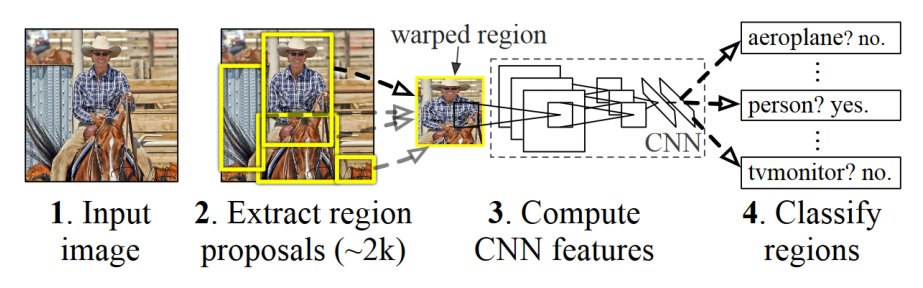
\includegraphics[width=0.85\linewidth]{figures/cnn/rcnn.eps}}
    \caption{Princip zpracování snímku pomocí R-CNN.\footnotemark}
    \label{fig:rcnn}
\end{figure}

\footnotetext{Převzato z~\cite{rcnn}.}

R-CNN využívá algoritmus selektivního hledání kandidátních oblastí představený v~prá-\\ci~\cite{selective-search}. Ta udává, že oblasti můžou obsahovat více informací než samotné pixely, proto by měly být při hledání upřednostňovány. Algoritmus je založen na nalezení několika počátečních oblastí a~následném iterativním shlukování oblastí (založeném na počítání podobnosti oblastí). Shlukování nejpodobnějších oblastí probíhá až do doby, kdy se celý snímek stane samostatnou oblastí. Protože algoritmus není invariantní vůči rozlišení vstupního snímku a~množství navržených oblastní závisí na jeho velikosti, musí se všem snímkům před provedením selektivního hledání změnit velikost na pevných $500\,\text{px}$.

Pro výpočet vstupního vektoru konvoluční sítě o~pevné délce z~navržené oblasti, nezávisle na jejím rozměru, se používá technika zvaná \emph{affine image warping}\footnotemark. Architektura konvoluční sítě má homogenní strukturu a~skládá se ze 13 konvolučních vrstev s~jádry o~velikosti $3 \times 3$. Mezi konvolučními vrstvami se nachází 5 maximalizačních sdružovacích vrstev a~architektura je zakončena třemi plně-propojenými vrstvami. Protože navržené oblasti mohou obsahovat jen část objektu, byl zvolen prah IoU $0.3$ -- pokud při validaci oblast překrývá \emph{ground-truth} o~méně než daný prah, je označena jako negativní. Při změně prahu na $0.5$ dojde k~poklesu mAP na datové sadě PASCAL VOC o~5 bodů \cite{rcnn}.

\footnotetext{\emph{Affine image warping} -- afinní obrazová deformace.}

Po získaní vlastností z~oblastí pomocí konvoluční sítě je použito jedno lineární SVM na každou třídu, které ohodnotí pravděpodobnost, zda vektor vlastností spadá do dané třídy. Poté je aplikováno potlačení ne-maximálních hodnot samostatně pro každou třídu, které ignoruje oblast, pokud má s~oblastí vyšší IoU, než je naučený prah.


\subsection*{Rychlejší verze -- Fast R-CNN}
\label{rcnnFast}
Ačkoli R-CNN dosahuje velmi dobré úspěšnosti detekce, doba vyhodnocení jednoho snímku trvá $\sim47$ sekund. Z~tohoto důvodu vznikly navazující verze Fast a~Faster (rychlá a~rychlejší) R-CNN. Zde je popsaná verze Fast R-CNN \cite{fast-rcnn}. Tato verze se snaží odstranit nevýhody R-CNN a~zároveň zvýšit rychlost a~úspěšnost detekce. Oproti R-CNN jsou během trénování upravovány všechny vrstvy, trénování je jedno-stupňové za použití více-úlohové ztrátové funkce a~extrahované vlastnosti už nejsou ukládány na disk.

Vstupem Fast R-CNN je vstupní snímek a~sada navržených oblastí, které jsou poté zpracovány, jak lze vidět na obrázku \ref{fig:fastrcnn}. Jako první je zpracován vstupní snímek pomocí několika konvolučních a~sdružovacích vrstev za účelem získání aktivační mapy. Poté jsou pro všechny navržené oblasti z~aktivačních map získány vektory vlastností pevné délky, které jsou posléze načteny do sady plně-propojených vrstev. Ty se poté větví do dvou posledních výstupních vrstev. Jedna slouží pro určení pravděpodobností jednotlivých tříd pomocí aktivační funkce softmax. Těchto tříd je celkem $K$ a~jedna specifická třída, která slouží k~odchycení veškerých detekcí pozadí. Druhá vrstva produkuje sadu 4 souřadnic predikovaných ohraničujících boxů pro každou z~$K$ tříd \cite{fast-rcnn}.

\begin{figure}[H]
    \centering
    \tmpframe{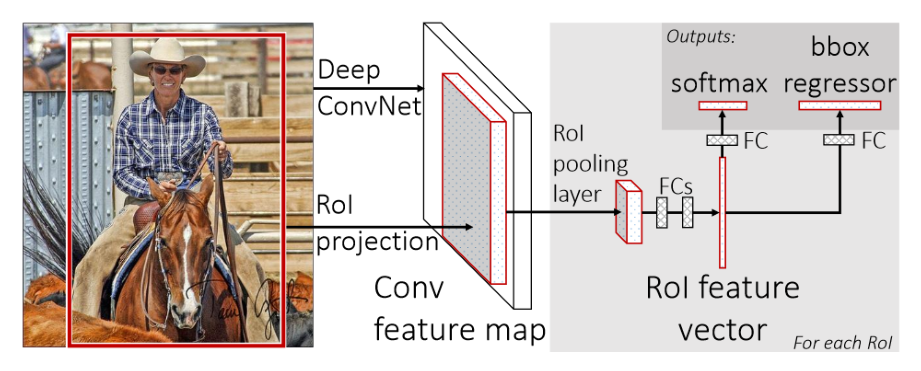
\includegraphics[width=0.85\linewidth]{figures/cnn/fastrcnn.eps}}
    \caption{Architektura systému Fast R-CNN.\footnotemark}
    \label{fig:fastrcnn}
\end{figure}

\footnotetext{Převzato z~\cite{fast-rcnn}.}

Výsledkem těchto úprav je, že:

\begin{itemize}
    \item Trénování Fast R-CNN je $9 \times$ rychlejší než trénování R-CNN.
    \item Detekce jednoho snímku provádí Fast R-CNN $213 \times$ rychleji.
    \item Na datové sadě PASCAL VOC 2012 dosahuje Fast R-CNN lepší úspěšnosti $66\,\%$ mAP (oproti $62\,\%$ R-CNN).
\end{itemize}